\chapter{结对编程与同行评审} % Introduction chapter suppressed from the table of contents

客户:我们的客户以银行为主,他们很注重质量,所以一直很注重评审。他们对需求评审、代码走查等也很赞同,也能找到缺陷,对提升质量有作用。但他们最困惑的是通过设计评审很难发现缺陷。\\
我:你听说过敏捷的结对编程吗?\\
客户:听过,也给客户做过培训,但是一般管理层都接受不了用两个人干一个人的活,所以几乎都没有团队在实际工作中使用。\\
我:当写完了几千行代码后,就很难在评审时要求开发改动。程序员会觉得又不是不对,测试也跑得通,为什么要改。所以代码的质量问题应在写的时候就避免,这是结对编程的原理。你可以把结对编程看成是一个提高团队之间互相交流的效率的工具。因为结对编程是在编码时针对具体问题集思广益进行解决,很容易落地,效果会比培训或评审好。\\
比如我跟另一位老师看一些团队的代码,他们都写了起码几千行。我们的结论就是:虽然代码的设计很有问题,但已经到了这个地步,除非重写,否则单靠修正部分代码并没有帮助。这也是设计评审常常难以做好的主要原因。而且大家都要面子,如果在评审里,直接说他设计有问题,也可能会影响到大家的关系,所以在设计评审时难以找出缺陷,这很正常。\\
客户:你说的很有道理,但为什么这二十年没有流行?\\
我:有很多人不了解怎样做好结对编程。例如:

\begin{itemize}
\tightlist
\item
  以为结对编程必须要找一位合适的搭档,人与人之间是否合得来最重要。
\item
  以为结对时只是在旁边看。
\item
  以为仅仅是培训,教同伴应怎么做。
\item
  以为只是看,作为人手编译器,只看代码是否写对,能否通过编译。
\end{itemize}

以上都并非结对编程的目的,也正因为这么多误解,才导致结对编程没有效果,后面就放弃了。代码规范很重要,你同意吗?\\
客户:同意。\\
我:代码规范本应是依据自己面对过的问题,形成清单,提醒自己要注意哪些问题------从实战中累积出来的检查请单,才有实用性。但很多团队的没有自己的代码规范,或只使用其他公司的。但如果团队结对编程,便能相互碰撞交流,可以更好地识别出规范应包括的检查项。\\
客户:我也很相信结对编程有用,但有什么好的方法去说服老板,得到他的支持。\\
我:你觉得结对编程后主要的好处是什么?\\
客户:代码的质量应该有所完善。\\
我:同意,但能否具体一点呢?例如之前有什么质量的问题影响项目客户。\\
客户:比如最近我们有个项目,测试都通过了,但是代码难以理解,读不懂。\\
我:同意,怎么解决这个问题?\\
客户:最终我们花费了大量时间对代码添加注释,还写了很多文档来解释。\\
我:后面加注释,添加支持类文档已经是亡羊补牢了,本该在写代码时就注意可读性。例如你觉得下面附件A与附件B代码,那种较好?\\
客户:附件A\\
我:其实附件A和附件B都没错,但附件A比附件B容易理解。所以如果团队用结对编程,就可以解决写代码时的质量问题,确保可读性。减少后面再后补文档或者再重构的时间。
如果你觉得代码可读性和后面难以维护是问题,让我们探索一下具体是什么问题,怎样解决。通常你们通过评审能发现多少问题(Bug)并在评审后修正、改善?\\
客户:几乎没有从评审找出可读性问题,我也带过一些初级的程序员,确实出现了不少这类问题,但项目时间很紧,我只能暴露那些最主要的大问题,这是可读性问题,确实很多时候就没有时间去处理了。\\
我:你可以估计一下,如果用了结对编程,要达到质量要求,后面可以节省返工。\\
客户:懂你的意思了,应该象前面 AP1
里那样,估算结对编程能为公司节省多少返工成本,并估计能带来多少回报。\\
我:是的,但估算节省时请注意不要误以为结对编程只能改善可读性,它只是其中一类。
客户:如老板也赞同,应该怎么开始?\\
我:因大家都从未试过,可以先做一天培训,先感受一下应如何结对编程。因为没有培训的话,很多原理大家还是无法弄懂。\\

\hypertarget{ux57f9ux8bad}{%
\subsection{培训}\label{ux57f9ux8bad}}

\hypertarget{ux7ed3ux5bf9ux7f16ux7a0bux76eeux6807}{%
\subsubsection{结对编程目标}\label{ux7ed3ux5bf9ux7f16ux7a0bux76eeux6807}}

\begin{itemize}
\tightlist
\item
  尽早识别问题,减少后面的返工。
\item
  促进知识分享和团队合作文化。
\item
  让两人可以相互协助。
\item
  同伴可放心评判对方的弱项。\\
\end{itemize}

\hypertarget{ux5148ux7528ux4ee3ux7801ux5b9eux4f8bux8ba9ux5b66ux5458ux4e86ux89e3ux5f53ux524dux7f16ux7801ux7684ux4e0dux8db3ux63d0ux51faux4ee5ux4e0bux6539ux8fdbux76eeux6807}{%
\subsubsection{先用代码实例让学员了解当前编码的不足,提出以下改进目标}\label{ux5148ux7528ux4ee3ux7801ux5b9eux4f8bux8ba9ux5b66ux5458ux4e86ux89e3ux5f53ux524dux7f16ux7801ux7684ux4e0dux8db3ux63d0ux51faux4ee5ux4e0bux6539ux8fdbux76eeux6807}}

\begin{itemize}
\tightlist
\item
  促进代码规范。
\item
  提高编码可读性。
\item
  方便后期复用。
\item
  有单元测试(测试驱动开发)。
\item
  更好了解需求。
\end{itemize}

\hypertarget{ux7528ux5c0fux7ec4ux4e92ux52a8ux7ec3ux4e60ux8ba9ux5b66ux5458ux4f53ux4f1aux4ee5ux4e0bux539fux5219}{%
\subsubsection{用小组互动练习,让学员体会以下原则}\label{ux7528ux5c0fux7ec4ux4e92ux52a8ux7ec3ux4e60ux8ba9ux5b66ux5458ux4f53ux4f1aux4ee5ux4e0bux539fux5219}}

\begin{enumerate}
\tightlist
\item
  一边编码一边说话。\\
\item
  不断的同步问问题,比如这个方法是否应放在这个类上面。\\
\item
  每个人都要带小本子和笔。\\
\item
  最后应该不断的重用、复用。\\
\end{enumerate}

\hypertarget{ux5de5ux5177}{%
\subsubsection{工具}\label{ux5de5ux5177}}

工作环境很重要,例如可以用一个大屏幕让两个人一起写和看代码:\\
%\href{文件:leip38.1.jpg}{600px}

\includegraphics[width=6cm]{leip381.jpg}

或者用Teamviewer共享工具,让两位程序员各自用自己一台笔记本电脑:\\
%\href{文件:leip38.2.png}{600px}

\includegraphics[width=6cm]{leip382.png}

\hypertarget{ux4e0dux4e00ux5b9aux5168ux7a0bux90fdux662fux7ed3ux5bf9ux53efux4ee5ux4e0eux5355ux72ecux4ea4ux66ff}{%
\subsubsection{不一定全程都是结对,可以与单独交替}\label{ux4e0dux4e00ux5b9aux5168ux7a0bux90fdux662fux7ed3ux5bf9ux53efux4ee5ux4e0eux5355ux72ecux4ea4ux66ff}}

%\href{文件:leip51.jpg}{500px}

\includegraphics[width=6cm]{leip51.jpg}

\hypertarget{ux4e0dux65adux66ffux6362}{%
\subsubsection{不断替换}\label{ux4e0dux65adux66ffux6362}}

如果结对编程总是由某一位编码,这容易开始,但是很难持续,这种互相分享知识的空间就越来越低。通常我们有好几种方式去对工作进行分工来做结对编程。例如最简单的是结对跟单独的交替或者共用跟私有结对等,也要考虑工位的安排。例如下图,有些座位可以让他们做到一起结对。另外有些是让他们私人做编程,减少干扰。\\
%\href{文件:Acp3-13.1.png}{400px}

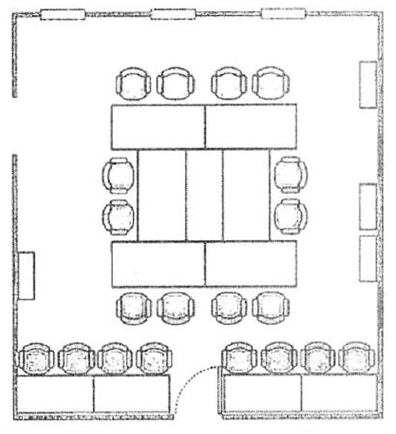
\includegraphics[width=6cm]{Acp3-131.png}

\hypertarget{ux57f9ux8badux540eux7684ux7ecfux9a8cux5206ux4eab}{%
\subsubsection{培训后的经验分享}\label{ux57f9ux8badux540eux7684ux7ecfux9a8cux5206ux4eab}}

培训的目的是让团队开始了解结对编程的精神:\\
\#我们先定一些小目标,例如提高代码的可读性。\\
\#改善变化,尽量让类可复用,而不是拷贝粘贴,然后尽量使用设计模式,而不是自己弄一个新的设计方法。

所以我们首先要有一个基本的代码规范,而且要求都写清楚。大家都了解以上原则后,可以让团队开始实战,通过练习感受结对编程的过程。很多时候学员都不习惯一边写代码,一边讲或者沟通,所以必须利用互动练习帮助学生提升这方面的能力。

\hypertarget{ux603bux7ed3}{%
\subsection{总结}\label{ux603bux7ed3}}

经过合适培训后,结对编程比评审更能有效地帮助团队写好代码,提高软件质量,并减少返工成本。\\
如老板赞同很多软件工程师经验少、没注意代码质量,导致后面大量返工,软件产品无法维护,我们除了可以以节省成本为由外,还可以用以下理由说服他:

\begin{itemize}
\tightlist
\item
  不是所有代码都结对编程,而是针对重要代码结对编程。例如项目初期搭建架构和写偏底层一些的代码,以及同类功能用于当样板的代码。
\item
  结对编程结对编程,因两人一起解决实际难题,很适合用于以老带新的工作方式,效果比讲解/培训好。
\end{itemize}

\hypertarget{ux9644ux4ef6}{%
\section{附件}\label{ux9644ux4ef6}}

\hypertarget{ux4ee3ux7801ux53efux8bfbux6027ux4f8bux5b50}{%
\subsection{代码可读性例子}\label{ux4ee3ux7801ux53efux8bfbux6027ux4f8bux5b50}}

%\href{文件:leip17.jpg}{600px}

%\href{文件:leip18.jpg}{600px}

%\href{文件:leip19.jpg}{600px}

\includegraphics[width=6cm]{leip17.jpg}

\includegraphics[width=6cm]{leip18.jpg}

\includegraphics[width=6cm]{leip19.jpg}




